\section{Lyttetests}
\fxnote{Generelt mere nær strukturen på noten. Udførlig argumentation for valg af testparametre.}
For at verificere hvor godt systemet virker, udføres en lyttetest på 9 antal vilkårlige testpersoner. Lyttetesten går ud på at de ud fra 10 specifikke testsignaler skal bedømme hvor de mener at lydkilden er placeret og notere både azimuth, elevation og distance. De 10 testsignaler er en blanding af speak og musik, hvor rækkefølgen er ABABA hvor A henviser til referencepunktet [1,0,0], og B henviser til den position som skal bestemmes af testpersonen. Hvert signal afspille i 10 sekunder.
Testen er udført med musikken afspillet fra en mobiltelefon (hhv en Huawei P10 Lite og en One Plus 2), og høretelefonerne er JBL Everest 300. Testpersonerne kunne afspille hvert testsignal så mange gange de ønskede. Signalerne er designet til at teste virkningsgraden af azimuth, elevation og distance, både hver for sig og i kombinationer. Derudover testes der på nogle psykoakustiske 'svære' placeringer, som f.eks. $180\deg$ azimuth eller $90\deg$ elevation.  
\fxnote{Obs på volumen og hvilken info de skal have LS}

%\begin{figure}[h!]
%	\centering
%	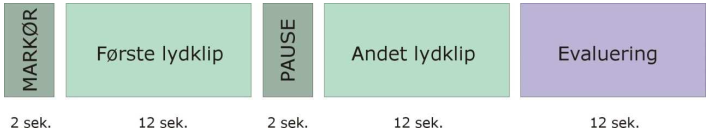
\includegraphics[width=0.7\linewidth]{All_Pics/ABtest}
%	\caption{}
%	\label{fig:abtest}
%\end{figure}
